\documentclass[a4paper, 12pt, twoside, openright]{article}
\newtheorem{theorem}{Twierdzenie}[section]
\usepackage[utf8]{inputenc}
\usepackage[T1]{polski}
\usepackage{helvet}
\usepackage{graphicx}
\usepackage{color}
\usepackage[cp1250]{inputenc}
\usepackage{subfig}
\usepackage[top=1.3in,bottom=1.3in,right=1in,left=1in,headheight=95pt,headsep=-0.5cm]{geometry}
\usepackage{color}
\usepackage{listings}
\usepackage{caption}
\newcounter{nalg}[subsection] % defines algorithm counter for chapter-level

\DeclareCaptionLabelFormat{algocaption}{Algorytm \thenalg} % defines a new caption label as Algorithm x.y
\lstnewenvironment{algorithm}[1][] %defines the algorithm listing environment
{   
	\refstepcounter{nalg}
	\captionsetup{labelformat=algocaption,labelsep=colon} 
	\lstset{ 
		mathescape=true,
		frame=tB,
		numbers=left, 
		numberstyle=\tiny,
		basicstyle=\scriptsize, 
		keywordstyle=\color{black}\bfseries\em,
		keywords={,input, output, return, datatype, function, in, if, else, foreach, while, begin, end, }
		numbers=left,
		xleftmargin=.04\textwidth,
		#1 
	}
}
{}



\begin{document}

\lstset{language=Python}
% =====  STRONA TYTULOWA  ====

\thispagestyle{empty}
\vspace*{-0.6in}
%% ------------------------ NAGLOWEK STRONY =======================------

\includegraphics[height=37.5mm]{logo_agh}\\
\rule{30mm}{0pt}
{\large\textsf{Wydział Fizyki i Informatyki Stosowanej}}\\
\rule{\textwidth}{3pt}\\
\rule[2ex]
{\textwidth}{1pt}\\
\vspace{7ex}
\begin{center}
{\bf\LARGE\textsf{Praca inżynierska}}\\
\vspace{13ex}
% ======================= IMIE I NAZWISKO =======================----
{\bf\Large\textsf{Klaudia Fil}}\\
\vspace{3ex}
{\sf \small kierunek studiów:} {\bf\small\textsf{informatyka stosowana}}\\
\vspace{15ex}
%% ------------------------ TYTUL PRACY =======================-----------
{\bf\huge\textsf{Problem chińskiego listonosza\\ w sieci ulic w Krakowie}}\\
\vspace{14ex}
%% ------------------------ OPIEKUN PRACY =======================---------
{\sf \Large Opiekun:} {\bf\Large\textsf{dr hab. inż. Przemysław Gawroński}}\\
\vspace{22ex}
\textsf{\bf\large\textsf{Kraków, styczeń 2021}}
\end{center}


\newpage

%% =====  Oświadczenie =========
\begin{center}
	{\bf\large\textsf{Oświadczenie studenta}}
\end{center}


{\sf 
	Uprzedzony(-a) o odpowiedzialności karnej na podstawie art. 115 ust. 1 i 2 ustawy z dnia 4 lutego 1994 r. o prawie autorskim i prawach pokrewnych (t.j. Dz. U. z 2018 r. poz. 1191 z późn. zm.): „Kto przywłaszcza sobie autorstwo albo wprowadza w błąd co do autorstwa całości lub części cudzego utworu albo artystycznego wykonania, podlega grzywnie, karze  ograniczenia wolności albo pozbawienia wolności do lat 3. Tej samej karze podlega, kto rozpowszechnia bez podania nazwiska lub pseudonimu twórcy cudzy utwór w wersji oryginalnej albo w postaci opracowania, artystyczne wykonanie albo publicznie zniekształca taki utwór, artystyczne wykonanie, fonogram, wideogram lub nadanie.”, a także uprzedzony(-a) o odpowiedzialności dyscyplinarnej na podstawie art. 307 ust. 1 ustawy z dnia 20 lipca 2018 r. Prawo o szkolnictwie wyższym i nauce (Dz. U. z 2018 r. poz. 1668 z późn. zm.) „Student podlega odpowiedzialności dyscyplinarnej za naruszenie przepisów obowiązujących w uczelni oraz za czyn uchybiający godności studenta.”, oświadczam, że niniejszą pracę dyplomową wykonałem(-am) osobiście i samodzielnie i nie korzystałem(-am) ze źródeł innych niż wymienione w pracy

\bigskip

	Jednocześnie Uczelnia informuje, że zgodnie z art. 15a ww. ustawy o prawie autorskim i prawach pokrewnych Uczelni przysługuje pierwszeństwo w opublikowaniu pracy dyplomowej studenta. Jeżeli Uczelnia nie opublikowała pracy dyplomowej w terminie 6 miesięcy od dnia jej obrony, autor może ją opublikować, chyba że praca jest częścią utworu zbiorowego. Ponadto Uczelnia jako podmiot, o którym mowa w art. 7 ust. 1 pkt 1 ustawy z dnia 20 lipca 2018 r. — Prawo o szkolnictwie wyższym i nauce (Dz. U. z 2018 r. poz. 1668 z późn. zm.), może korzystać bez wynagrodzenia i bez konieczności uzyskania zgody autora z utworu stworzonego przez studenta w wyniku wykonywania obowiązków związanych z odbywaniem studiów, udostępniać utwór ministrowi właściwemu do spraw szkolnictwa wyższego i nauki oraz korzystać z utworów znajdujących się w prowadzonych przez niego bazach danych, w celu sprawdzania z wykorzystaniem systemu antyplagiatowego. Minister właściwy do spraw szkolnictwa wyższego i nauki może korzystać z prac dyplomowych znajdujących się w prowadzonych przez niego bazach danych w zakresie niezbędnym do zapewnienia prawidłowego utrzymania i rozwoju tych baz oraz współpracujących z nimi systemów informatycznych.}

\vspace{15ex}

\begin{center}
\begin{tabular}{lr}
~~~~~~~~~~~~~~~~~~~~~~~~~~~~~~~~~~~~~~~~~~~~~~~~~~~~~~~~~~~~~~~~~ &
................................................................. \\
~ & {\sf (czytelny podpis)} \\
\end{tabular}
\end{center}

%% =====  TYL STRONY TYTULOWEJ   ====


%% ============ OCENA OPIEKUNA =============
\newpage
\linespread{1.3}
\selectfont

\hspace*{\fill}\large{Ocena merytoryczna opiekuna}

\vspace{85mm}

%% ============ OCENA RECENZENTA =============
\newpage
\linespread{1.3}
\selectfont

\hspace*{\fill}\large{Ocena merytoryczna recenzenta}

\vspace{85mm}


%% ====== SPIS TRESCI ==========
\newpage
\tableofcontents


%=======================- 1 =======================
\newpage
\section{Wstęp}
\subsection{Wprowadzenie}
	\indent\par
	Szeroko pojęty problem związany z wyznaczaniem trasy (ang. General Routing Problem) zdefiniowano jako szukanie drogi o minimalnym koszcie, która dodatkowo musi spełniać uwzględnione w planowaniu wymagania$^{\cite{varianntsCPP}}$.
	Skupiając się na praktycznym aspekcie GRP należy wziąć pod uwagę jeden z bardziej znanych przypadków rozważań - problem chińskiego listonosza (ang.Chinese Postman Problem)$^{\cite{arcRoutingProblemsPart1}}$. 


	W życiu codziennym wiele zawodów związanych jest wyznaczaniem trasy na tle procesów logistycznych, wśród nich różnego rodzaju dostawca, kurier czy właśnie listonosz. Ich szlakiem docelowym jest droga zawierająca w sobie każdą ulicę danego obszaru przynajmniej raz. Optymalnym rozwiązaniem CPP byłoby uniknięcie ponownych przejść jedną ścieżką, jednak w sytuacjach rzeczywistych jest to często niemożliwe.

\subsection{Cel pracy}
	\indent\par
	Celem pracy dyplomowej jest zaimplementowanie dwóch algorytmów, rozwiązujących kwestię znajdowania pełnej ścieżki z cyklem zamkniętym na grafie spójnym, przy optymalizacji kosztów przemieszczania się, co sprowadza się do CPP. 
	Rozpatrzono w niej przypadki rzeczywiste, gdzie w powstałych z mapy Krakowa grafach mieszanych (ang. Mixed Graph) oraz nieskierowanych (ang. Undirected Graph), znajdowana jest najlepsza droga dla listonosza$^{\cite{mixedGraph}}$.


	Jeden z algorytmów przedstawiony w pracy dedykowany jest MG. Swoje zastosowanie ma, kiedy przebieg trasy listonosza uwarunkowany jest czynnikami zewnętrznymi tj. drogami jedno- lub dwukierunkowymi. 
	W przypadku pieszego ruchu, w którym sposób przejścia jest  dowolny, problem dotyczy UG. Zaimplementowano dla niego drugi z schematów umożliwiający wyznaczenie najbardziej efektywnej trasy. Graf rzeczywisty tworzony jest z małych fragmentów miasta, dlatego założono, że poruszać się będzie na nim tylko jeden listonosz. 


	Dla sprawdzenia poprawności oraz wyznaczenia złożoności algorytmów wygenerowano losowe sieci, które umożliwiły szersze ich przetestowanie. 
	Stworzono również program do wizualizacji grafów, oraz kolejnych etapów ścieżek, umożliwiający graficzne prześledzenie działania schematów.




\subsection{Problemu chińskiego listonosza}
	\indent\par
	Problem chińskiego listonosza jest jedynym z podstawowych zagadnień związanych z wyznaczaniem trasy. Swoją nazwę zawdzięcza chińskiemu matematykowi, który jako pierwszy go sformułował. Analizował drogę dostawcy w jednym z chińskich miast, który miał dostarczyć wszystkie przesyłki, odwiedzając każdą ulice, nie nadkładając niepotrzebnie drogi i powrócić do bazy$^{{\cite{CPP}}}$. 
	
	Patrząc przez pryzmat przypadku rzeczywistego, gdzie rozważany jest listonosz, czy dostawca ulotek, CPP sprowadza się do procesu wyboru najlepszej ścieżki w sieci dróg, gdzie  każda ulica musi zostać odwiedzona przynajmniej raz, czyli odnalezienia na grafie cyklu Eulera$^{\cite{MatchingEulertourAsCPP}}$. 

\subsection{Cykl Eulera} \label{SciezkaEulera}

\indent\par
	Cykl Eulera (ang. Eulerian Cycle) jest to ścieżka poprowadzona na dowolnym grafie, która przechodzi przez każdą z krawędzi dokładnie raz. Nazywamy ją cyklem, ponieważ zaczyna się i kończy w tym samym wierzchołku. 
	
	Nazwa takiego przejścia przez graf nadana została na cześć matematyka Leonharda Eulera, który w swojej pracy \textit{Solutio problematis ad geometriam situs pertinentis}$^{\cite{euler}}$ poruszył zagadnienie mostów królewieckich. Odpowiadał na pytanie, czy istnieje ścieżka prowadząca przez wszystkie mosty, biorąc pod uwagę, że przez każdy z nich można iść tylko raz. 
	
	\begin{figure}[htb]
		\centering
		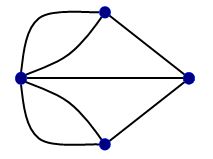
\includegraphics[width=0.5\textwidth]{WSTEP1}
		\caption[]{Graf przestawiający problem mostów w Królewcu}
		\label{krolewiec}
	\end{figure}

	Mapa, którą rozważał, sprowadzała się do grafu z rysunku \ref{krolewiec}, gdzie krawędzie odpowiadają siedmiu mostom. Wykazał, że znalezienie EC jest możliwe tylko dla grafów spełniających określone warunki, nazwanych na jego cześć grafami Eulera. Była to jedna z pierwszych prac związanych z teorią grafów.
	
	\subsubsection{Graf Eulera}
	\begin{theorem}[Euler, 1736]
		\label{twEuleraUG}
		Graf spójny jest eulerowski wtedy i tylko wtedy, gdy
		stopień każdego wierzchołka jest liczbą parzystą.	
	\end{theorem}

	 \begin{theorem}
	 	\label{twEuleraDG}
	 	Graf skierowany spójny zawiera cykl Eulera wtedy i tylko wtedy, gdy
	 	dla każdego wierzchołka v zachodzi $d ^{+} (v) = d ^{-} (v) $, gdzie \indent\par$d ^{+} (v)$ - ilość krawędzi wchodzących do wierzchołka v, \indent\par$d ^{-} (v)$ - ilość krawędzi wychodzących z wierzchołka v.
	 \end{theorem}
 
	 Aby możliwe było znalezienie poprawnej ścieżki dzięki opisanym w tej pracy algorytmom, grafy w nich wykorzystywane muszą spełniać twierdzenia \ref{twEuleraUG} i \ref{twEuleraDG}. 
	 
	 W przypadku wygenerowania UG niezgodnego z \ref{twEuleraUG} wywoływana jest funkcja odpowiedzialna za dodanie duplikatów krawędzi, które zapewnią poprawny stopnień każdego z wierzchołków. Wierzchołki o nieparzystych stopniach dobierane są w możliwie najlepsze pary (wykorzystując algorytm najkrótszych ścieżek) i łączone ze sobą. 
	 
	 Analogiczna sytuacja jest dla DG w odniesieniu do twierdzenia \ref{twEuleraDG}. 
	 

\subsection{Sieci złożone} \label{SieciZlozone}
\subsubsection{Sieć Barabási–Albert}
\indent\par

 	Pod koniec XX w. na Uniwersytecie Notre Dame w Indianie Reka Albert i Albert-Laszlo Barabasi podczas badania struktury sieci WWW przypadkiem odkryli ciekawą zależność, a mianowicie potęgowe rozkłady prawdopodobieństwa opisujące połączenia pomiędzy stronami internetowymi.
 
	 Rozkład ten wyglądał następująco:
 	\begin{equation}
 		\label{eqn:rozkladP}
 		P(k) \sim k ^{-\alpha}
 	\end{equation}
 	co oznaczało, że sieć WWW ma własności fraktalne.

 	Zauważono, że większość układów rzeczywistych również charakteryzuje się rozkładem podobnym do równania \ref{eqn:rozkladP}. Szerszą analizę i reguły tworzenia sieci tego typu Panowie przedstawili w swojej pracy zatytułowanej \textit{Emergence of scaling in random networks}$^{\cite{barabasiAlbert}}$. Ustalili, że rozkład \ref{eqn:rozkladP} wynika z wzrostu sieci i reguły związanej z preferencyjnym dołączaniem węzłów.
 	
 
 
	Formułowanie ewoluującej sieci polega na stopniowym jej rozroście w każdym momencie czasowym. Proces rozpoczęty w chwili zerowej składa się z grafu zawierającego $m_0$ połączonych wierzchołków. Podczas kolejnych kroków czasowych nowo dodawany węzeł łączony jest z $m$ innymi, istniejącymi już. Szansa, że świeżo utworzony wierzchołek połączony zostanie krawędzią do starego węzła jest proporcjonalne do stopnia węzła $k_i$:
	
	\begin{equation}
		\Pi (k_i) = { k_i \over {\sum_{i=1}^{t} k_i} }
	\end{equation}
	co przedstawione jest na rysunku \ref{BarabasiImg1}.
	
		\begin{figure}[!hbt]
		\centering
		\subfloat[$m=1$, $t=3$]{\label{b_a}
			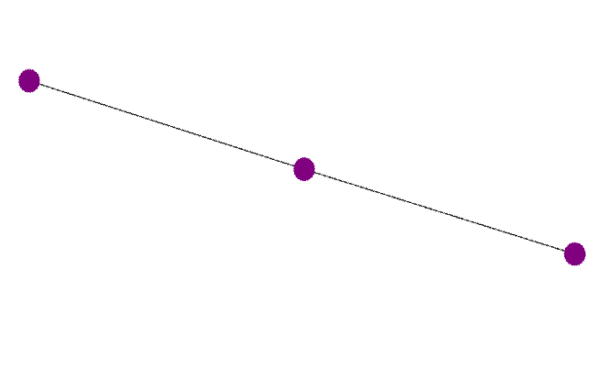
\includegraphics[width=0.4\textwidth]{bara_1a.png}}
		\quad
		\subfloat[$m=1$, $t=6$]{\label{b_b}
			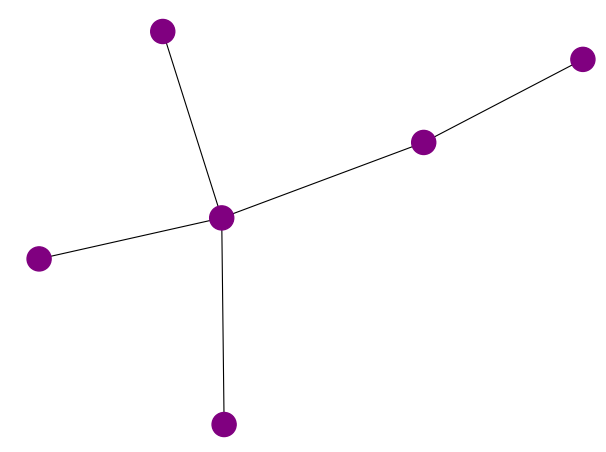
\includegraphics[width=0.4\textwidth]{bara_1b.png}}
		\quad
		\subfloat[$m=1$, $t=10$]{\label{b_c}
			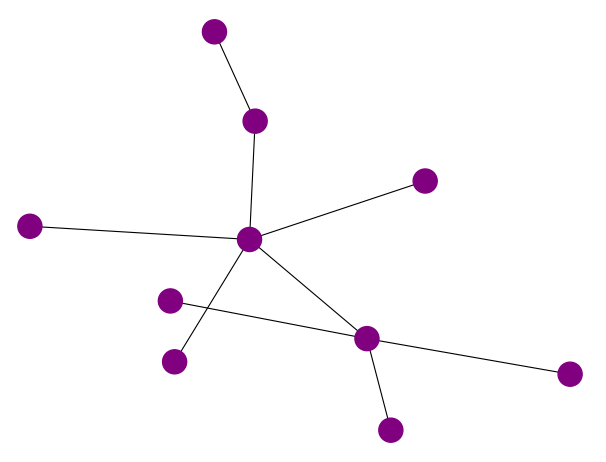
\includegraphics[width=0.4\textwidth]{bara_1c.png}}
		\quad
		\subfloat[$m=1$, $t=15$]{\label{b_d}
			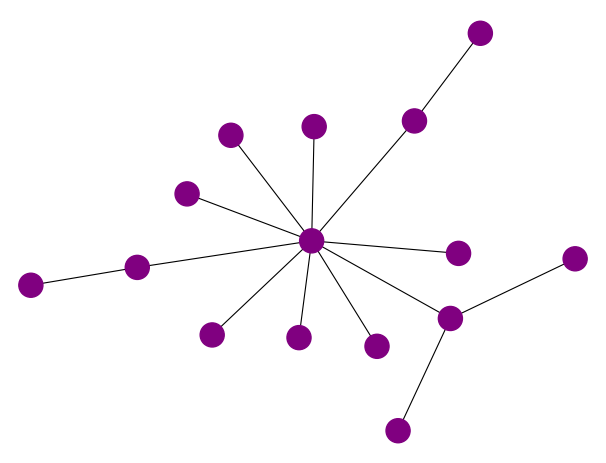
\includegraphics[width=0.4\textwidth]{bara_1d.png}}
		
		\caption[]{Graf losowy stworzony zgodnie z modelem Barabási–Albert}
		\label{BarabasiImg1}
	\end{figure}
 	
 	
 	Algorytm posiłkowy, z którego skorzystano w pracy, tworzący grafy w wyżej opisanym modelu to \textit{barabasi\char`_albert\char`_graph}, zaczerpnięto go z biblioteki \textit{Networkx} szerzej opisanej w rozdziale \ref{narzedzia}.
	
	
\subsubsection{Sieć Watts–Strogatz}
\indent\par
Zjawiskiem małego świata tylko dla pewnego ograniczonego zakresu, zależnie od wielkości sieci.$^{\cite{samllWorld}}$

% ======================= 2 =======================
\newpage
\section{Narzędzia} \label{narzedzia}

\indent\par
	Aplikacja w całości została zaimplementowana w Pythonie, ze względu na jego prostotę i czytelność, które ułatwiały znacznie pracę. Innym atrybutem przemawiającym za tym językiem jest duża ilość bibliotek związanych z teorią grafów. Jedna z nich została wykorzystana przy tworzeniu projektu, m. in. do wyliczania najkrótszych ścieżek, ale również przy tworzeniu losowych grafów.

Biblioteki użyte w pracy:
\begin{itemize}
	\item \textit{Networkx}$^{\cite{networkx}}$ - biblioteka w języku Python używana przy badaniu i tworzeniu dużych grafów i sieci. Wykorzystana została w algorytmie konwertującym graf do takiego, który posiada ścieżkę Eulera opisaną w \ref{SciezkaEulera} i podczas tworzenia przypadkowego digrafu oraz sieci złożonych z podpunktu \ref{SieciZlozone}.
	\item \textit{Matplotlib}$^{\cite{matplotlib}}$ - jedna z najbogatszych bibliotek do tworzenia wykresów w języku Python. W pracy gównie wykorzystano zawarte w niej API \textit{pylab} wykorzystujące prosty interface analogiczny do środowiska MATLAB$^{\cite{matlab}}$.
\end{itemize}

	Inną istotną rzeczą użytą w projekcie to mapa świata OpenStreetMap (OSM)$^{\cite{openstreetmap}}$, która zbudowana jest z danych gromadzonych przez szeroką społeczność. Dowolna osoba może przyczynić się do jej rozwoju poprzez dostarczenie informacji geograficznych zbieranych przez urządzenia z odbiornikami GPS lub zdjęcia satelitarne. Dane w niej są udostępnione za darmo do ogólnego użytku.




%======================= 3 =======================
\newpage
\section{Algorytmy i implementacja}

\subsection{Modyfikacja do grafu Eulera}
\subsubsection{Modyfikacja grafu nieskierowanego}
\indent\par
dddd
\begin{algorithm}[caption={\textit{makeEulerianGraph} przekształcający graf nieskierowany do grafu Eulera}, label={makeeulerianUG}]
def makeEulerianGraph(graph):
	listOfOddDegreeNodes = []
	
	for node in graph.nodes(data=True):
		if idOddNumber(graph.degree[node[0]]):
			listOfOddDegreeNodes.append(node[0])
	
	if idOddNumber(len(listOfOddDegreeNodes)):
		return None
	
	listOfOddDegreeNodes1 = listOfOddDegreeNodes[:len(listOfOddDegreeNodes) // 2]
	listOfOddDegreeNodes2 = listOfOddDegreeNodes[len(listOfOddDegreeNodes) // 2:]
	listOfRandomParams = list()
	
	for x in range(0, 100):
		random.shuffle(listOfOddDegreeNodes2)
		listOfRandomParams.append(list(zip(listOfOddDegreeNodes1, 
							listOfOddDegreeNodes2)))
							
	minPath = getOptimalAdditionalPaths(graph, listOfRandomParams)
	appendFakeEdges(graph, minPath)
\end{algorithm}
sddd
\subsubsection{Modyfikacja grafu skierowanego}
\indent\par
dddd

\begin{algorithm}[caption={\textit{makeEulerianDiGraph} przekształcający graf skierowany do grafu Eulera}, label={makeeulerianDG}]
def makeEulerianDiGraph(graph):
	diff = [None] * len(
			graph.nodes)  # list with nodes difference : 
			    	      # predecessors nodes - successors nodes
	for node in graph.nodes(data=True):
		diff[node[0]] = len(graph.pred[node[0]]) - len(graph.succ[node[0]])
	
	negNodes = []
	posNodes = []
	for node in range(0, len(diff)):
		if diff[node] < 0:
			for rep in range(-1 * diff[node]):
				negNodes.append(node)
		if diff[node] > 0:
			for rep in range(diff[node]):
				posNodes.append(node)
	
	if idOddNumber(len(negNodes) - len(posNodes)):
		return None
	
	listOfRandomParams = list()
	
	for x in range(0, 100):
		random.shuffle(negNodes)
		listOfRandomParams.append(list(zip(posNodes, negNodes)))
	
	minPath = getOptimalAdditionalPaths(graph, listOfRandomParams)
	appendFakeEdges(graph, minPath)   
\end{algorithm}
sddd


\subsection{Graf rzeczywisty}\label{grafRzecz}
\indent\par
Algorytmy docelowo szukają optymalnej trasy na planie miasta Kraków. Poprawne ich zastosowanie wymaga konwersji mapy na postać grafową. 

\begin{figure}[htb]
	\centering
	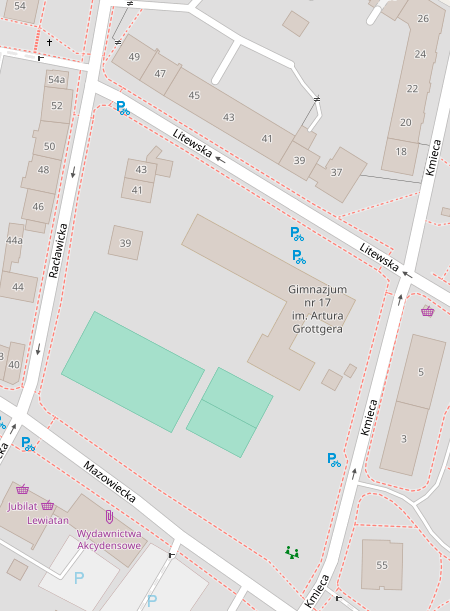
\includegraphics[width=0.5\textwidth]{OSM1}
	\caption[]{Fragment mapy Krakowa\footnotemark}
	\label{osm1}
\end{figure}

\footnotetext{Zrzut ekranu z strony https://www.openstreetmap.org/}

Przetwarzając mapę z rysunku \ref{osm1} formujemy graf, którego krawędzie odpowiadają ulicom, a wierzchołki reprezentują zarówno budynki, jak i istotne elementy dróg: skrzyżowania i strategiczne punkty trasy, które to potrzebne są do idealnego przeprowadzenia ulicy, czyli uwzględnienia zakrętów lub nieliniowych fragmentów drogi.

\begin{figure}[htb]
	\centering
	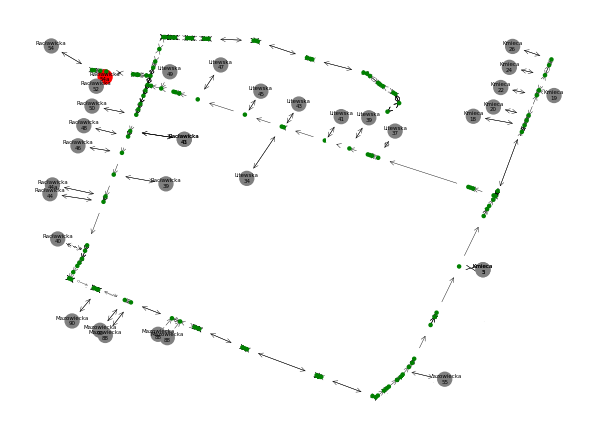
\includegraphics[width=0.9\textwidth]{OSM1graf}
	\caption[]{Graf rzeczywisty MG stworzony z mapy z rysunku \ref{osm1}}
	\label{osm1G}
\end{figure}

Program odpowiedzialny za generowanie grafu, przy pobieraniu danych z bazy OpenStreetMap, filtruje odpowiednie informacje o obiektach i znajduje placówkę pocztową (o ile taka istnieje na danych fragmencie miasta) dzięki konkretnym tagom\cite{osmPropertis}. W przypadku wybrania fragmentu mapy, gdzie nie ma poczty, to miano nadawane jest losowo wybranej nieruchomości.

Wierzchołki w grafie podpisano rzeczywistymi adresami oraz oznaczono różnymi kolorami, w celu zwiększenia czytelności. Placówkę pocztową przedstawiono na czerwono, zwykłe budynki mieszkalne na szaro. Natomiast wierzchołki będące fragmentami drogi pokolorowano na zielono oraz zmniejszono ich rozmiar względem pozostałych.

Analizując kierunki dróg na rysunku \ref{osm1}. można zauważyć, że wpływają one na budowę grafu rzeczywistego z rysunku \ref{osm1G}, który w przypadku kiedy listonosz porusza się np. samochodem jest MG. Dla pieszej podróży  określono go jako UG.

\subsection{Implementacja grafu rzeczywistego}
\indent\par
........................

\subsection{Algorytm Fleury’ego}
\indent\par
........................

\begin{algorithm}[caption={\textit{FleuryAlgorithm} wyszukujący ścieżkę w grafie nieskierowanym}, label={makeeulerianDG}]
def FleuryAlgorithm(graph, startNode):
	adjList = GraphHelper.getAdjList(graph)
	EulerCycle = list()
	
	findNextNode(adjList, startNode, EulerCycle)
	return EulerCycle
\end{algorithm}

\begin{algorithm}[caption={\textit{findNextNode} rekurencyjna funkcja pomocnicza dla \textit{FleuryAlgorithm} }, label={makeeulerianDG}]
def findNextNode(adjList, n, EulerCycle):
	EulerCycle.append(n)
	for v in adjList[n]:
		if isBridge(adjList, n, v):
			removeEdge(adjList, n, v)
			findNextNode(adjList, v, EulerCycle)
\end{algorithm}

\begin{algorithm}[caption={\textit{findNextNode} rekurencyjna funkcja pomocnicza dla \textit{FleuryAlgorithm} }, label={makeeulerianDG}]
def isBridge(adjList, u, v):
	if len(adjList[u]) == 1:
		return True
	else:
		listOfVisitedNeighbours = [False] * len(adjList)
		cntBeforeRestoreEdge = DFS(adjList, u, listOfVisitedNeighbours)
		
		removeEdge(adjList, u, v)
		listOfVisitedNeighbours = [False] * len(adjList)
		cntAfterRestoreEdge = DFS(adjList, u, listOfVisitedNeighbours)
		
		# restore edge
		addEdge(adjList, u, v)
		
		return cntBeforeRestoreEdge < cntAfterRestoreEdge

\end{algorithm}

\subsection{Algorytm Hierholzera}
\indent\par
........................
\captionsetup{justification=centering}
\begin{algorithm}[caption={\textit{HierholzerAlgorithm} funkcja wyznaczająca ścieżkę dla grafów skierowanych i nieskierowanych }, label={makeeulerianDG}]
def HierholzerAlgorithm(graph, isDirected, startNode):
	adjList = GraphHelper.getAdjList(graph)
	EulerCycle = list()
	stackOfNodes = deque()
	
	node = startNode
	EulerCycle.append(node)
	
	while True:
		if checkOutDegree(adjList, node):
			v = getNextOutEdge(adjList, node)
			stackOfNodes.append(node)
			removeEdge(adjList, node, v, isDirected)
			node = v
		else:
			node = stackOfNodes.pop()
			EulerCycle.append(node)
		
		if not stackOfNodes:
			break
		
	EulerCycle.reverse()
	return EulerCycle
\end{algorithm}



% ======================= 4 =======================
\newpage
\section{Wyniki}
\par\indent
........................



% ======================= 5 =======================
\newpage
\section{Podsumowanie}
\indent\par
........................



% ======================= LITERATURA =======================
\newpage
\bibliographystyle{srt}
\begin{thebibliography}{99}
	
	% 1.1
	\bibitem{varianntsCPP}
		M.K. Gordenko, S.M. Avdoshin \textit{The Variants of Chinese Postman Problems and Way of Solving through Transformation into Vehicle Routing Problems.} Trudy ISP RAN/Proc. ISP RAS, vol. 30, issue 3, s. 221-232, 2018
	
	\bibitem{arcRoutingProblemsPart1}
		H. A. Eiselt, M. Gendreau, G. Laporte, \textit{Arc Routing Problems, Part I: The Chinese Postman Problem}  Institute for Operations Research and the Management Sciences (INFORMS), 1995
	
	\bibitem{mixedGraph}
		M. Beck, D. Blado, J. Crawford, T. Jean-Louis, M. Young \textit{On weak chromatic polynomials of mixed graphs}, Graphs and Combinatorics, 2013

	% 1.3	
	\bibitem{CPP} 
		R. K. Ahuja, T. L. Magnanti, J. B. Orlin \textit{Network  Flows:  Theory,  algorithmsand applications}, Prentice Hall, New Jersey, s. 740-745, 1993
	
	\bibitem{MatchingEulertourAsCPP} 
		J. Edmonds, E.L. Johnson \textit{Matching Euler tours and the Chinese postman problem}. Mathematical Programming, s. 88–124, 1973
	
	% 1.4
	\bibitem{euler} 
		Leonhard Euler \textit{Solutio problematis ad geometriam situs pertinentis} (ang.), 1741
	
	%\bibitem{mixedNetworksCPP} 
	%	W.L. Pearn, J.B. Chou. \textit{Improved solutions for the Chinese postman problem on mixed networks}. Computers\&Operations Research, s. 819–827, 1999
	
	% 1.5
	\bibitem{barabasiAlbert}
	A.-L. Barabási, R. Albert \textit{Emergence of Scaling in Random Networks}, Science 286, 509-512, 1999

	
	%%%%%%%%%%%%%%%%%%
	
	\bibitem{samllWorld}
	K. Klemm, V. M. Eguiluz \textit{Growing scale-free networks with small-world behavior},
	Physical Review , vol. 65, 057102, 2002
	
	\bibitem{swiatSieciZlozonych}
	A. Fronczak, P. Fronczak \textit{Świat sieci złożonych. Od fizyki do Internetu}, Wydawnictwo
	Naukowe PWN, 2009

	
%	\bibitem{cormen}
%		Thomas H. Cormen, Charles E. Leiserson, Ronald L. Rivest, Clifford Stein, \textit{Wprowadzenie do algorytmów}, Wydawnictwo Naukowe PWN, Warszawa 2012

	% 2
	\bibitem{python} https://pl.python.org/ [dostęp: 23.12.2020]
	
	\bibitem{networkx} https://networkx.org/ [dostęp: 23.12.2020]
	
	\bibitem{matplotlib} https://matplotlib.org/ [dostęp: 23.12.2020]

	\bibitem{matlab} https://www.mathworks.com/help/matlab/ [dostęp: 23.12.2020]
	
	\bibitem{openstreetmap} https://www.openstreetmap.org/ [dostęp: 23.12.2020]
	
	
	%%%%%%%%
	\bibitem{osmPropertis} https://wiki.openstreetmap.org/wiki/Category:Properties 
	
	[dostęp: 20.12.2020]

\end{thebibliography}	


\end{document}
